\documentclass[10pt,a4paper]{article}
\usepackage[T1]{fontenc}
\usepackage[utf8]{inputenc}
\usepackage[left=0.5cm, right=0.5cm, top=0.5cm, bottom=0.5cm]{geometry}
\geometry{verbose}
\usepackage{multicol}
\usepackage{titlesec}
\usepackage{setspace}
\usepackage{enumitem}
\usepackage{fontawesome5}
\usepackage{xcolor}
\usepackage{graphicx}

\usepackage[scaled]{helvet}
\renewcommand{\familydefault}{\sfdefault}

\titleformat{\section}{\large\bfseries}{}{0em}{}

\titlespacing{\section}{0pt}{5pt}{2pt}

\newcommand{\myvspace}{\vspace{0.3cm}}
\newcommand{\myvspaceSection}{\vspace{0.7cm}}

\definecolor{blanc}{rgb}{1,1,1}
\definecolor{VertClair}{rgb}{0.627451,0.72549,0.694118}
\definecolor{CouleurSection}{rgb}{0.188235,0.313726,0.376471}
\definecolor{CouleurClair}{rgb}{0.937255,0.937255,0.937255}
\definecolor{noir}{rgb}{0,0,0}

\titleformat{\section}
  {\color{CouleurSection}\normalfont\normalsize\bfseries} % Couleur et style
  {\thesection}{1em}{}

\begin{document}

\noindent\small
\colorbox{CouleurSection}{
    \begin{minipage}[t]{0.2\textwidth}
        \vspace{0pt} % Align text to the top
        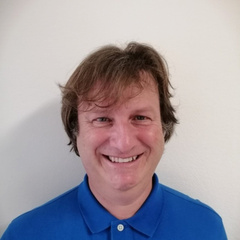
\includegraphics[trim=20 0 20 20, clip, width=80pt]{latexImage_88a9fb5666ec9dfaab7b36fadf8aaf2a.png}
    \end{minipage}
    \begin{minipage}[t]{0.78\textwidth} 
        \vspace{15pt} % Align text to the top
        {\Huge \textbf{\textcolor{blanc}Christophe Maggiore}}\\
        \vspace{10pt}
        {\LARGE \textcolor{blanc}Développeur Informatique | Testeur Logiciel}\\
        \vspace{3pt}
        {\large  \textcolor{blanc}Business Central / Dynamics NAV}
    \end{minipage}
}
\noindent{}
\begin{minipage}[t]{0.30\textwidth}
\vspace{0pt}
% Colonne de gauche
\fcolorbox{VertClair}{VertClair}{
    % \begin{minipage}{\textwidth}
    \noindent\begin{minipage}[c]{1\textwidth}%
    \myvspaceSection
    \section*{\textcolor{noir}{email=christophe.maggiore@libertysurf.fr, telephone=06 61 56 83 85, ville=Nice}}
        \begin{spacing}{2}
            {\large \faEnvelope}\: \textbf{christophe.maggiore@libertysurf.fr} \\
            {\large \faPhone}\: \textbf{06 61 56 83 85} \\
            {\large \faMapMarker}\: \textbf{Nice} \\
            {\large \faCar}\: \textbf{Permis B}
        \end{spacing}
    \end{minipage}
}

\colorbox{CouleurClair}{
\begin{minipage}{\textwidth}
    \myvspaceSection
    \section*{{certifications=[{nom=Scrum Developer, etat=En cours}, {nom=ISTQB Foundation, etat=Acquise}], techniques={ERP=[Microsoft Dynamics NAV, Business Central], outils=[GitHub, Selenium, Squash TM, JUnit5], frameworks=[Spring, Angular, Bootstrap], langages=[Java, TypeScript, SQL, Python, VBA, AL], bases_de_donnees=[SQL Server, Access], methodologies=[Agile (Scrum), Test-driven development (TDD)]}}}
    \begin{itemize}[nosep, leftmargin=*, itemsep=0pt, parsep=0pt]
        \myvspace
        \item \textbf{Certification scrum developer (en cours)}
        \myvspace
        \item \textbf{Certification testeur logiciels: ISTQB foundation}
        \myvspace
        \item \textbf{Microsoft Dynamics NAV / Business Central}: Développement, Migration, Installation, Module de Tests
        \myvspace
        \item \textbf{Outils}: GitHub, Selenium, Squash TM, JUnit5
        \myvspace
        \item \textbf{Framework}: Spring, Angular, Bootstrap
        \myvspace
        \item \textbf{Langage}:Java, TypeScript, SQL, Python, VBA, AL
        \myvspace
        \item \textbf{Base de données}: SQL Server, T-SQL,Access
        \myvspace
        \item \textbf{Méthodes}:Agile (Scrum), Test-driven, development (TDD)
    \end{itemize}
    \myvspaceSection
    \section*{{francais=natif, anglais=intermédiaire}}
    \begin{itemize}[nosep, leftmargin=*, itemsep=0pt, parsep=0pt]
        \item Français (natif)
        \item Anglais (intermédiaire)
    \end{itemize}
    \myvspaceSection
    \section*{[Diplomatie, Autonome, Dynamique, Bon relationnel, Esprit d’équipe]}
    \begin{itemize}[nosep, leftmargin=*, itemsep=0pt, parsep=0pt]
        \item Diplomatie
        \item Autonome
        \item Dynamique
        \item Bon relationnel
        \item Esprit d’équipe
    \end{itemize}
    \myvspaceSection
    \section*{[Natation, Monopalme, Théâtre, Musique, Lecture, Voyages (États-Unis, Australie, Costa Rica), Conception de sites Web]}
    \begin{itemize}[nosep, leftmargin=*, itemsep=0pt, parsep=0pt]
        \item Pratique natation, monopalme, théâtre, musique, lecture
        \item Voyages (États-Unis, Australie, Costa Rica)
        \item Conception de sites Web
    \end{itemize}
    \myvspace
    \myvspace
    \myvspace
    \myvspace
\end{minipage}
\vspace{2cm}
}
\end{minipage}
\hfill{}
\indent
\begin{minipage}[t]{0.65\textwidth}
    \vspace{10pt}
    \hspace{0.7cm}Après plusieurs années d’expérience dans le développement informatique en particulier dans les domaines de la gestion et de la finance, je suis passionné par la création de solutions logicielles innovantes qui favorisent la réussite financière des entreprises tout en répondant à leurs besoins opérationnels. Mon objectif est de mettre mes compétences au service de votre entreprise, et je suis disponible dès maintenant pour rejoindre votre équipe.
    % Colonne de droite : Expériences professionnelles
    \myvspace
    \section*{[{annee=2024, poste=Développeur JAVA J2EE, entreprise=POEC IB Cegos, taches=[Web Services, Développement avec Spring, Angular, TypeScript, Bootstrap, Participation aux phases de spécifications et de tests, Accès aux données SQL]}, {periode=2020 - 2023, poste=Développeur, entreprise=ELYSYS, Monaco, description=Société d’édition et de service informatique spécialisé dans l’industrie financière (Télétravail hybride), taches=[Développement d’extensions Microsoft Dynamics 365 Business Central, PowerShell, VBA, Langage de programmation AL, environnement de développement : Visual Studio Code, Réalisation de tests automatisés de la solution, Mise en production et upgrades de la solution]}, {periode=2018 - 2020, poste=Développeur, entreprise=KEESYSTEM, Monaco, taches=[Développement avec FileMaker Pro, Système de gestion financière de portefeuilles automatisé (Pour gérants indépendants, family offices et banques privées)]}, {annee=2017, poste=Développeur, entreprise=ALLIGATOR ESN, taches=[Sage module logistique, maintenance, corrections, PL-SQL]}, {periode=2004 - 2017, poste=Développeur, entreprise=ELYSYS, Monaco, taches=[Développement MS Dynamics NAV, T-SQL, VBA, Développement de système de gestion comptable/financière, Analyse et force de proposition de solutions techniques, Gestion des tests et de la qualité, maîtrise des releases, Développement et mise en production de solutions spécifiques pour divers clients, Expérience sur des projets orientés finance (Banques privées, sociétés de gestion, Family offices)]}, {periode=2002 - 2004, poste=Développeur, entreprise=BELLE ALLURE Communication, Nice, taches=[Développement VB 6.0, et VB.Net, Logiciels d’aide au diagnostic relooking, gestion des vendeurs et des produits]}, {periode=1999 - 2002, poste=Développeur, entreprise=SOLSI-CONSEIL, Monaco, taches=[Développement VB 6.0, VBA, Access 97 et 2000, Réalisation d’Add-ons pour une suite logicielle de comptabilité/paye et spécifiques, Maintenance informatique (installation de logiciels, matériels, réseaux)]}]}

    \textbf{2024 - Développeur JAVA J2EE (POEC IB Cegos) }
    \begin{itemize}[nosep, leftmargin=*, itemsep=0pt, parsep=0pt]
            \item Web Services 
            \item Développement avec Spring, Angular, TypeScript, Bootstrap 
            \item Participation aux phases de spécifications et de tests 
            \item Accès aux données SQL
    \end{itemize}
    \myvspace
    \textbf{2020/2023 ELYSYS, Monaco, Société d’édition et de service
    informatique spécialisé dans l’industrie financière (Télétravail hybride)
    Développement d’extensions Microsoft Dynamics 365 Business Central,
    PowerShell, VBA}
    \begin{itemize}[nosep, leftmargin=*, itemsep=0pt, parsep=0pt]
    \item Langage de programmation AL, environnement de développement : Visual Studio
    Code
    \item \textbf{\textit{Réalisation de tests automatisés de la solution}}
    \item Mise en production et upgrades de la solution
    \end{itemize}
    \myvspace
    
    \textbf{2018/2020 KEESYSTEM, Monaco \\
    Développement avec FileMaker Pro} 
        \begin{itemize}[nosep, leftmargin=*, itemsep=0pt, parsep=0pt]
            \item Système de gestion financière de portefeuilles automatisé, ( Pour gérants
        indépendants , family offices et banques privées ). 
        \end{itemize}
    \myvspace
    \textbf{2017 ALLIGATOR ESN} 
        \begin{itemize}[nosep, leftmargin=*, itemsep=0pt, parsep=0pt]
            \item Sage module logistique, maintenance, corrections, PL-SQL 
        \end{itemize}
    \myvspace
    \textbf{2004/2017 ELYSYS, Monaco \\
    Développement MS Dynamics NAV , T-SQL, VBA} 
    \begin{itemize}[nosep, leftmargin=*, itemsep=0pt, parsep=0pt]
        \item Développement au sein de l’équipe R\&D – Activité édition logiciel :
            \begin{itemize}[nosep, leftmargin=*, itemsep=0pt, parsep=0pt]
                \item[$\circ$] Développement de système de gestion comptable/financière
                \item[$\circ$] Analyse, force de proposition solution technique
                \item[$\circ$] Prise en charge complète des développements
                \item[$\circ$] Gestion des tests, Gestion de la qualité, Maîtrise des releases
            \end{itemize}
        \item Développement pour l’équipe ‘projet’ – Développements spécifiques :
            \begin{itemize}[nosep, leftmargin=*, itemsep=0pt, parsep=0pt]
                \item[$\circ$] Développement et mise en production de solutions spécifiques pour divers
                clients.
                \item[$\circ$] Expérience sur une multitude de projets orientés finance (Banques privés,
                \item[$\circ$] société de gestion, Family, offices)
            \end{itemize}
    \end{itemize}
    \myvspace
    \textbf{2002/2004 BELLE ALLURE Communication, Nice \\
    Développement VB 6.0, et VB.Net. }
        \begin{itemize}[nosep, leftmargin=*, itemsep=0pt, parsep=0pt]
            \item Logiciels d’aide au diagnostic relooking, gestion des vendeurs et des produits 
        \end{itemize}
    \myvspace 
    \textbf{1999/2002 SOLSI-CONSEIL, Monaco \\
    Développement VB 6.0, VBA, Access 97 et 2000. }
        \begin{itemize}[nosep, leftmargin=*, itemsep=0pt, parsep=0pt]
            \item Réalisation d’Add-ons pour une suite logicielle de comptabilité/paye et spécifiques.
            \item Maintenance informatique (installation de logiciels, matériels, réseaux)
        \end{itemize}
    \myvspace
    \section*{[{annee=2024, intitule=Développeur JAVA J2EE, organisme=POEC IB Cegos}, {annee=2024, intitule=Formation Testeur Logiciel, organisme=POEC, Antibes}, {intitule=DEUST Informatique, Sciences de l’Homme et de la Société, organisme=UFR - Nice - Sophia Antipolis}]}
    \begin{itemize}[nosep, leftmargin=*, itemsep=0pt, parsep=0pt]
        \item \textbf{2024} - Développeur JAVA J2EE (POEC IB Cegos)
        \item \textbf{2024} - Formation Testeur Logiciel (POEC, Antibes) 
        \item \textbf{DEUST Informatique}, Sciences de l’Homme et de la Société (UFR - Nice - Sophia Antipolis)
    \end{itemize}

\end{minipage}

\end{document}
